\documentclass[journal]{IEEEtran}
\usepackage[utf8]{inputenc}
\usepackage[spanish]{babel} 
\usepackage{graphicx}
\usepackage{amsmath}
\usepackage{siunitx}
\usepackage{hyperref}
\usepackage{url}
\usepackage{cite}
\hyphenation{op-tical net-works semi-conduc-tor}

\begin{document}
	
	\title{Laboratorio 1: Características eléctricas de las compuertas lógicas}
	\author{Jonathan, Mariano}
	\date{Febrero 2021}
	
	\newcommand{\email}[1]{\href{mailto:#1}{#1}}
	
	\author{
		\IEEEauthorblockN
		{
			Jonathan Guzmán Araya,
			Mariano Muñoz Masís
		}
		\IEEEauthorblockA{\\Instituto Tecnológico de Costa Rica}
		\IEEEauthorblockA{\\Área Académica Ingeniería en Computadores}
		
		\IEEEauthorblockA{\email{jonathana1196@gmail.com}}
		\IEEEauthorblockA{\email{marianomm1301@gmail.com}}
	}
	
	% The paper headers
	\markboth{Laboratorio Taller de Diseño Digital, Semestre I~2021}%
	{Shell \MakeLowercase{\textit{et al.}}: Bare Demo of IEEEtran.cls for IEEE Journals}
	
	
	% make the title area
	\maketitle
	
	% As a general rule, do not put math, special symbols or citations
	% in the abstract or keywords.
	\begin{abstract}
		The logic gates are built by semiconductor devices and taking into account their own specifications, these will have different functional characteristics that will make them belong to one or another family of logic gates.
		Each family has advantages one over the other, depending on the application that is needed, the one that best suits is selected, although they can also be combined through interfaces to achieve more specific applications.
	\end{abstract}
	
	% Note that keywords are not normally used for peerreview papers.
	\begin{IEEEkeywords}
		Arreglos, compuerta lógica, interfaz, NPN, PNP, tensión, transistor.
	\end{IEEEkeywords}
	
	\IEEEpeerreviewmaketitle
	
	\section{Introducción}
	\IEEEPARstart{E}{l} siguiente informe de laboratorio tiene como objetivo acercar al estudiante a las realidades que puede enfrentar en las practicas de campo en cuanto al comportamiento eléctrico de las compuertas de las familias Lógica Transistor-Transistor llamadas comúnmente por sus siglas en inglés TTL y las compuertas Metal-óxido-semiconductor complementario llamadas CMOS, además de guiar al estudiante al uso de herramientas y dispositivos relacionados con estos dispositivos.
	
	Las Compuertas Lógicas son circuitos electrónicos conformados internamente por transistores que se encuentran con arreglos especiales con los que otorgan señales de voltaje como resultado o una salida de forma booleana, están obtenidos por operaciones lógicas binarias (suma, multiplicación). También niegan, afirman, incluyen o excluyen según sus propiedades lógicas \cite{LOGICBUS}.
	
	\vspace{5mm}
	
	Existen diferentes tipos de compuertas y algunas son más complejas, con la posibilidad de ser simuladas por compuertas más sencillas, algunas de estas compuertas lógicas son:
	
	\begin{itemize}
		
		\item AND: Esta compuerta es representada por una multiplicación en álgebra de Boole, lo que indica que es necesario que en todas sus entradas se tenga un estado binario 1 (positivo) para que la salida genere un 1 binario. En caso contrario de que falte alguna de sus entradas con este estado o no tenga si quiera una accionada, la salida no podrá cambiar de estado y permanecerá en 0 (negativo) \cite{LOGICBUS}.
		
		\begin{table}[ht]
			\centering
			\begin{tabular}{|c|c|c|}
				\hline
				A & B & Q \\
				\hline
				\hline
				0 & 0 & 0 \\
				\hline
				0 & 1 & 0 \\
				\hline
				1 & 0 & 0 \\
				\hline
				1 & 1 & 1 \\
				\hline
			\end{tabular}
			\caption{Tabla de verdad de la compuerta AND}
			\label{tab:AND}
		\end{table}
		
		\begin{figure}[!htb]
			\centering
			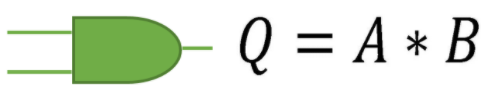
\includegraphics[scale = 0.3]{img/AND.png}
			\caption{Compuerta AND y su representación en álgebra de Boole \cite{LOGICBUS}}
			\label{fig:AND}
		\end{figure}
		
		\item NAND: También denominada como AND negada, esta compuerta trabaja al contrario de una AND ya que al no tener entradas en 1 o solamente alguna de ellas, esta concede un 1 en su salida, pero si esta tiene todas sus entradas en 1 la salida se presenta con un 0 \cite{LOGICBUS}.
		
		\begin{table}[ht]
			\centering
			\begin{tabular}{|c|c|c|}
				\hline
				A & B & Q \\
				\hline
				\hline
				0 & 0 & 1 \\
				\hline
				0 & 1 & 1 \\
				\hline
				1 & 0 & 1 \\
				\hline
				1 & 1 & 0 \\
				\hline
			\end{tabular}
			\caption{Tabla de verdad de la compuerta NAND}
			\label{tab:NAND}
		\end{table}
		
		\begin{figure}[!htb]
			\centering
			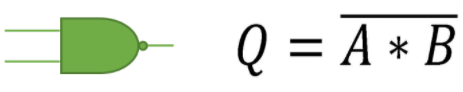
\includegraphics[scale = 0.35]{img/NAND.png}
			\caption{Compuerta NAND y su representación en álgebra de Boole \cite{LOGICBUS}}
			\label{fig:NAND}
		\end{figure}
		
		\item OR: En el álgebra de Boole esta es una suma. Esta compuerta permite que con cualquiera de sus entradas que este en estado binario 1, su salida pasara a un estado 1 también. No es necesario que todas sus entradas estén accionadas para conseguir un estado 1 a la salida pero tampoco causa algún inconveniente. Para lograr un estado 0 a la salida, todas sus entradas deben estar en el mismo valor de 0 \cite{LOGICBUS}.
		
		\begin{table}[ht]
			\centering
			\begin{tabular}{|c|c|c|}
				\hline
				A & B & Q \\
				\hline
				\hline
				0 & 0 & 0 \\
				\hline
				0 & 1 & 1 \\
				\hline
				1 & 0 & 1 \\
				\hline
				1 & 1 & 1 \\
				\hline
			\end{tabular}
			\caption{Tabla de verdad de la compuerta OR}
			\label{tab:OR}
		\end{table}
		
		\begin{figure}[ht]
			\centering
			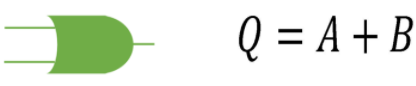
\includegraphics[scale = 0.35]{img/OR.png}
			\caption{Compuerta OR y su representación en álgebra de Boole \cite{LOGICBUS}}
			\label{fig:OR}
		\end{figure}
		
		\item NOT: Esta compuerta solo tiene una entrada y una salida, actúa como un inversor \cite{LOGICBUS}.
		
		\begin{table}[ht]
			\centering
			\begin{tabular}{|c|c|}
				\hline
				Q & Q' \\
				\hline
				\hline
				0 & 1 \\
				\hline
				1 & 0 \\
				\hline
			\end{tabular}
			\caption{Tabla de verdad de la compuerta NOT}
			\label{tab:NOT}
		\end{table}
		
		\begin{figure}[!htb]
			\centering
			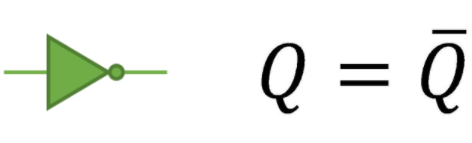
\includegraphics[scale = 0.35]{img/NOT.png}
			\caption{Compuerta NOT y su representación en álgebra de Boole \cite{LOGICBUS}}
			\label{fig:NOT}
		\end{figure}
		
		\item XOR: También llamada OR exclusiva, esta actúa como una suma binaria de un dígito cada uno y el resultado de la suma seria la salida. Otra manera de verlo es que con valores de entrada igual el estado de salida es 0 y con valores de entrada diferente, la salida será 1 \cite{LOGICBUS}.
		
		\begin{table}[ht]
			\centering
			\begin{tabular}{|c|c|c|}
				\hline
				A & B & Q \\
				\hline
				\hline
				0 & 0 & 0 \\
				\hline
				0 & 1 & 1 \\
				\hline
				1 & 0 & 1 \\
				\hline
				1 & 1 & 0 \\
				\hline
			\end{tabular}
			\caption{Tabla de verdad de la compuerta XOR}
			\label{tab:XOR}
		\end{table}
		
		\begin{figure}[!htb]
			\centering
			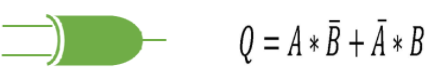
\includegraphics[scale = 0.4]{img/XOR.png}
			\caption{Compuerta XOR y su representación en álgebra de Boole \cite{LOGICBUS}}
			\label{fig:XOR}
		\end{figure}
		
	\end{itemize}
	
	\vspace{4mm}
	
	A diferencia de una compuerta lógica ideal, una compuerta lógica real debe ajustarse a la naturaleza de los elementos y materiales que la componen, dando así origen a las familias lógicas.
	Una familia lógica es un grupo de dispositivos que comparten un tecnología común de fabricación y tienen estandarizadas sus características de entrada y de salida; es decir son compatibles entre sí.
	
	\subsection{Alimentación CD}
	Tanto la familia TTL como la CMOS requieren de un voltaje de alimentación para funcionar, en el caso de la familia TTL el voltaje de alimentación CD ($V_{CC}$) es de +5 V, y la familia CMOS tiene distintos valores de voltaje de alimentación ($V_{DD}$) +5 V, +3.3 V, +2.5 V y +1.2 V. 
	\subsection{Significado de Términos}
	Indistintamente de la familia las compuertas trabajan con "0's" y "1's" lógicos, para representar el estado ALTO (HIGH) o el estado BAJO (LOW), la distinción se hace en el termino de "rango de valores admitidos", de esta manera es importante definir los términos $V_{IL}$, $V_{IH}$, $V_{OL}$ y $V_{OH}$.
	\vspace{6mm}
	\begin{itemize}
		\item $V_{IL}$ : Rango de tensiones de entrada que representan un nivel bajo.
		\item $V_{IH}$ : Rango de tensiones de entrada que representan un nivel alto. 
		\item $V_{OL}$ : Rango de tensiones de salida que representan un nivel bajo.
		\item $V_{OH}$ : Rango de tensiones de salida que representan un nivel alto.
	\end{itemize}
	
	\begin{table}[htb]
		\centering
		\begin{tabular}{llll}
			\hline
			& CMOS 5V & CMOS 3.3V & TTL \\
			\hline
			$V_{IH}$ máx. &  5      & 3.3        & 5 \\
			$V_{IH}$ mín. &  3.5    & 2          & 2 \\
			$V_{IL}$ máx. &  1.5    & 0.8        & 0.8 \\
			$V_{IL}$ mín. &  0      & 0          & 0 \\
		\end{tabular}
		\caption{Valores nominales de tensión de entrada para cada tecnología}
		\label{tab:VInput}
	\end{table}
	
	\begin{table}[htb]
		\centering
		\begin{tabular}{llll}
			\hline
			& CMOS 5V & CMOS 3.3V & TTL \\
			\hline
			$V_{OH}$ máx. &  5      & 3.3        & 5 \\
			$V_{OH}$ mín. &  4.4    & 2.4        & 2.5 \\
			$V_{OL}$ máx. &  0.33   & 0.4        & 0.4 \\
			$V_{OL}$ mín. &  0      & 0          & 0 \\
		\end{tabular}
		\caption{Valores nominales de tensión salida para cada tecnología}
		\label{tab:VOutput}
	\end{table}
	
	\subsection{Fan-out y Fan-in}
	Otro término que se debe conocer es el \textsl{fan-out}, básicamente este término se refiere a la cantidad de compuertas lógicos que se pueden conectar a la salida de una compuerta lógica. Se determina de la siguiente manera: 
	
	\begin{equation}
		fan-out=\frac{I_{OH}}{I_{IH}}
	\end{equation}
	
	\begin{equation}
		fan-out=\frac{I_{OL}}{I_{IL}}
	\end{equation}
	
	Tomando como referencia el valor mas pequeño de las ecuaciones (1) y (2). Este valor es de suma importancia, ya que nos indica que cantidad de compuertas se puede manejar con las corrientes en Alto y en Bajo, para evitar daños en los componentes. 
	
	\subsection{Interfaces}
	Conocer a fondo ambas tecnologías nos permite realizar circuitos que ayuden a mejorar los tiempos de propagación y disminuir la potencia disipada.
	La tecnología CMOS ofrece ventajas en cuanto a la tensión de alimentación, la temperatura de trabajo, inmunidad al ruido, el fan-out y potencia disipada, por su lado la tecnología TTL presenta ventajas con un menor tiempo de conmutación y un costo ligeramente más bajo.
	
	\vspace{5mm}
	
	Además, según las ventajas que ofrece cada tecnología se pueden realizar interfaces. Una interfaz es la interconexión eficiente de dos dispositivos, circuitos o sistemas que no son compatibles entre sí y tiene características eléctricas diferentes. Las interfaces lógicas permiten que dispositivos de diferentes familias puedan comunicarse satisfactoriamente entre sí. 
	
	\vspace{5mm}
	
	Una entrada CMOS es relativamente fácil de manejar a partir de una salida TTL cuando los dispositivos involucrados en la interfaz operan a partir de una misma fuente de $+5 V$. Las características de corriente de salida de TTL son más que adecuadas para manejar entradas CMOS, solo deben hacerse compatibles los niveles de tensión. Entre los tipos de interfaces posibles de TTL a CMOS y viceversa tenemos:
	
	\begin{figure}[!htb]
		\centering
		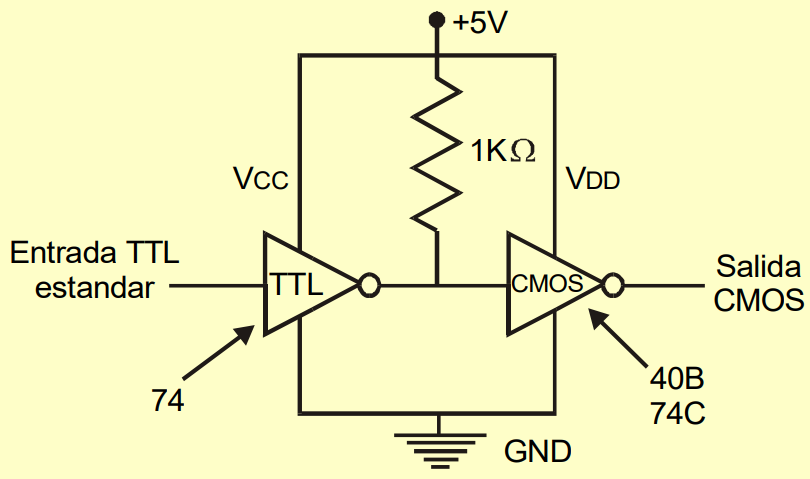
\includegraphics[scale = 0.25]{img/TTLCMOSRes.png}
		\caption{Interfaz TTL a CMOS con resistencia \cite{Ladelex}}
		\label{fig:TTLCMOSRes}
	\end{figure}
	
	\begin{figure}[!htb]
		\centering
		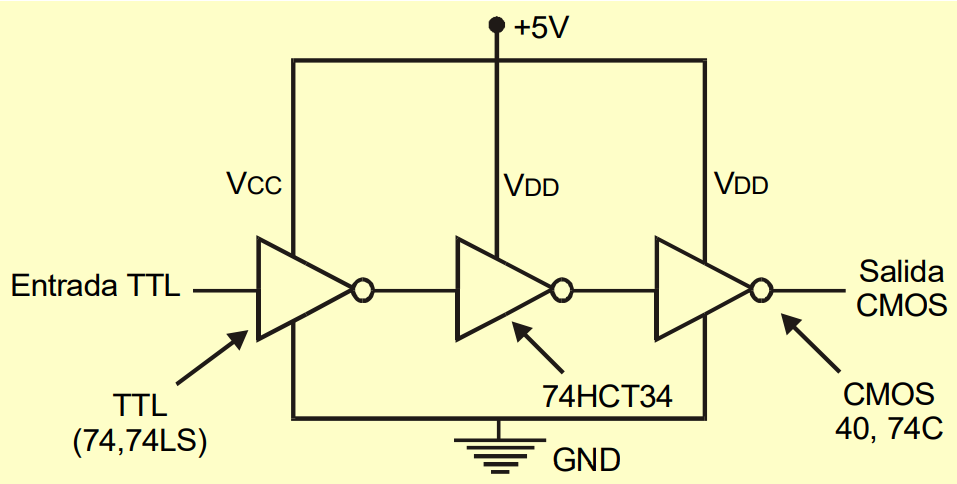
\includegraphics[scale = 0.25]{img/TTLCMOS74HC.png}
		\caption{Interfaz TTL a CMOS con 74HCT34 \cite{Ladelex}}
		\label{fig:TTLCMO74HC}
	\end{figure}
	
	\begin{figure}[!htb]
		\centering
		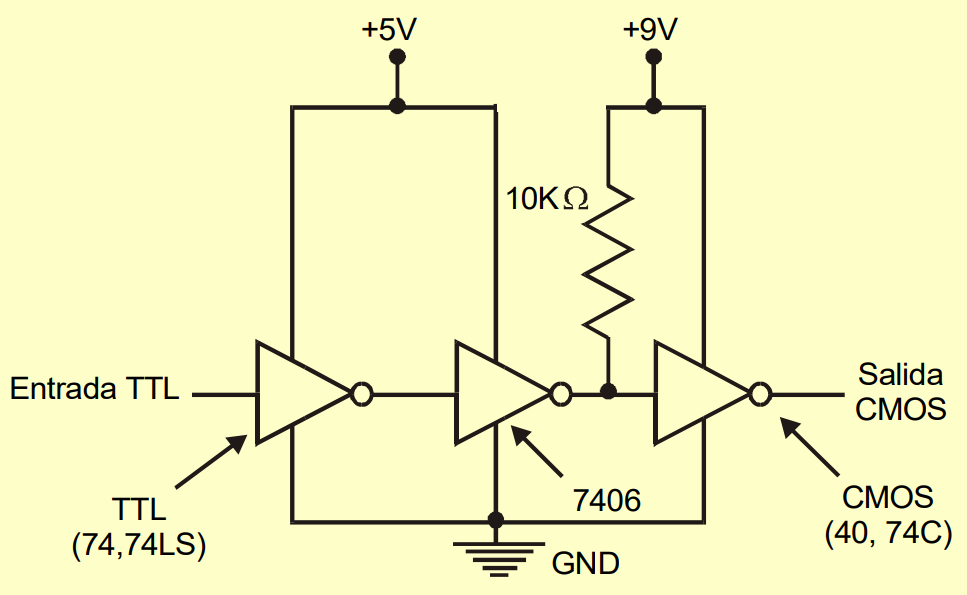
\includegraphics[scale = 0.25]{img/TTLCMOSColAb.png}
		\caption{Interfaz TTL a CMOS con colector abierto \cite{Ladelex}}
		\label{fig:TTLCMOSColAb}
	\end{figure}
	
	\begin{figure}[!htb]
		\centering
		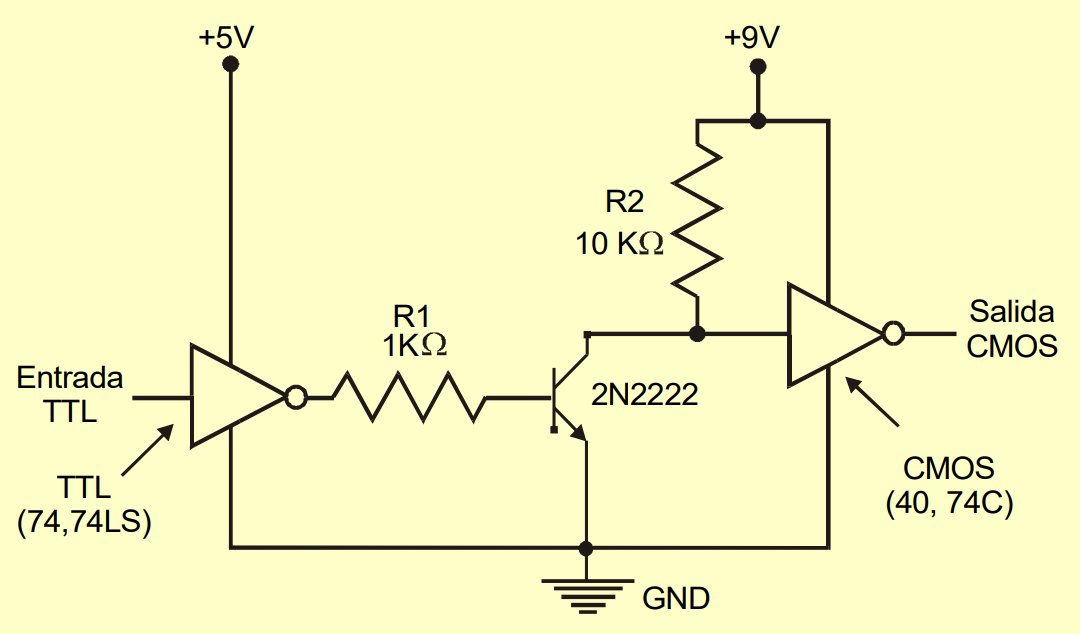
\includegraphics[scale = 0.25]{img/TTLCMOSTrans.png}
		\caption{Interfaz TTL a CMOS con transistor \cite{Ladelex}}
		\label{fig:TTLCMOSTrans}
	\end{figure}
	
	\begin{figure}[!htb]
		\centering
		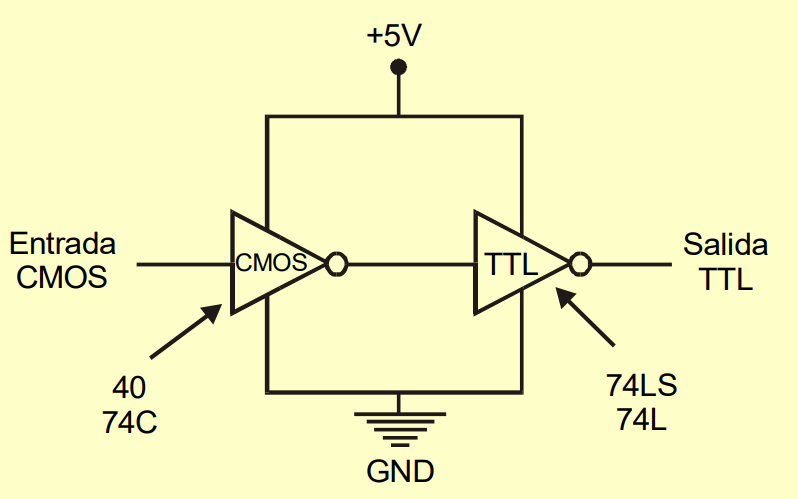
\includegraphics[scale = 0.25]{img/CMOSTTL.png}
		\caption{Interfaz directa CMOS a TTL \cite{Ladelex}}
		\label{fig:CMOSTTL}
	\end{figure}
	
	\begin{figure}[htb]
		\centering
		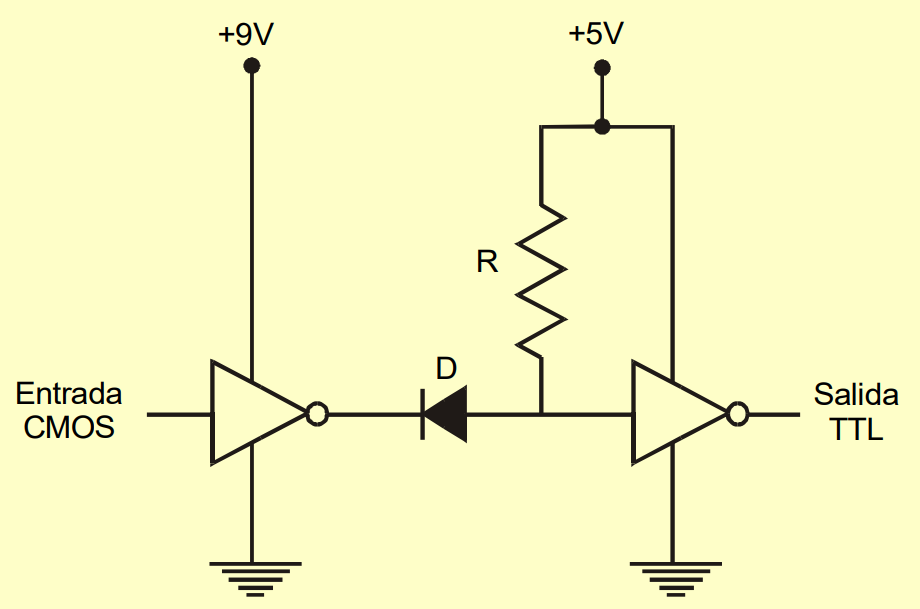
\includegraphics[scale = 0.25]{img/CMOSTTLRes.png}
		\caption{Interfaz CMOS a TTL con resistencia \cite{Ladelex}}
		\label{fig:CMOSTTLRes}
	\end{figure}
	
	\begin{figure}[!htb]
		\centering
		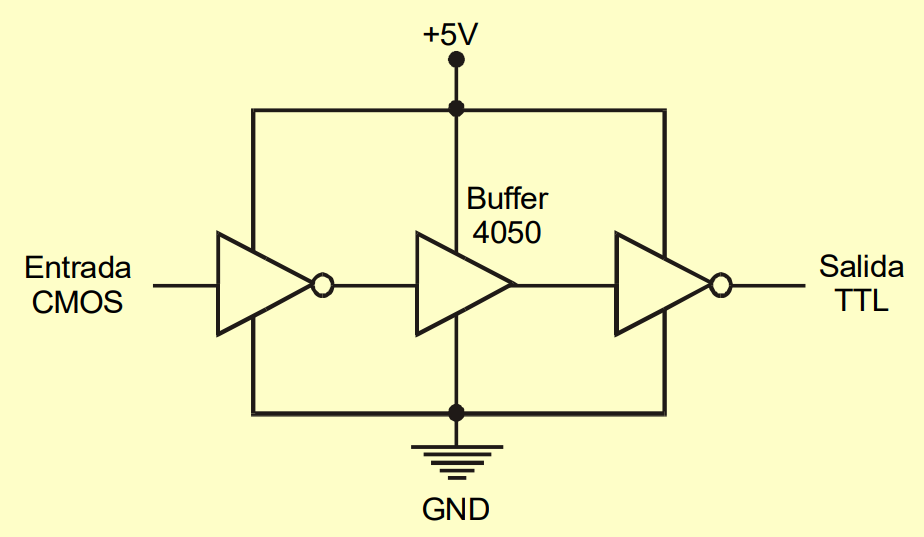
\includegraphics[scale = 0.25]{img/CMOSTTLBuff.png}
		\caption{Interfaz CMOS a TTL con buffer CMOS \cite{Ladelex}}
		\label{fig:CMOSTTLBuff}
	\end{figure}
	
	\begin{figure}[!htb]
		\centering
		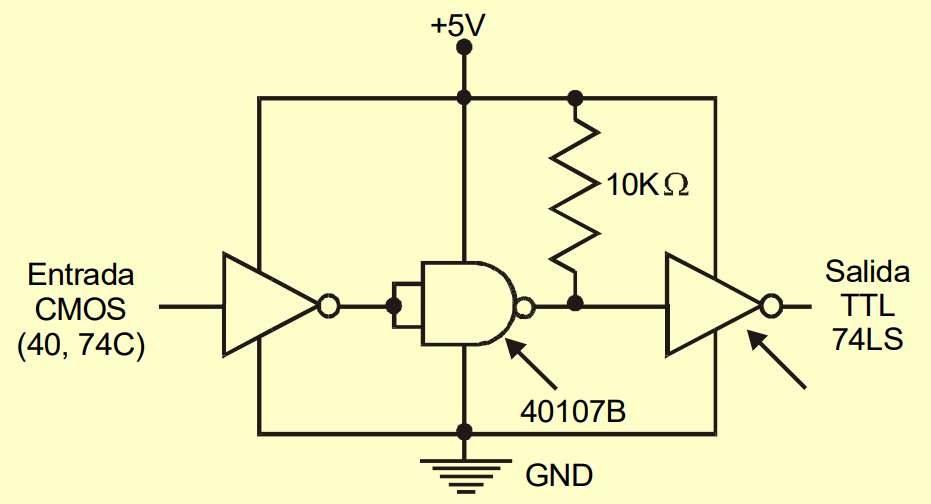
\includegraphics[scale = 0.25]{img/CMOSTTL40.png}
		\caption{Interfaz de CMOS a TTL con 40107B \cite{Ladelex}}
		\label{fig:CMOSTTL40}
	\end{figure}
	
	\begin{figure}[!htb]
		\centering
		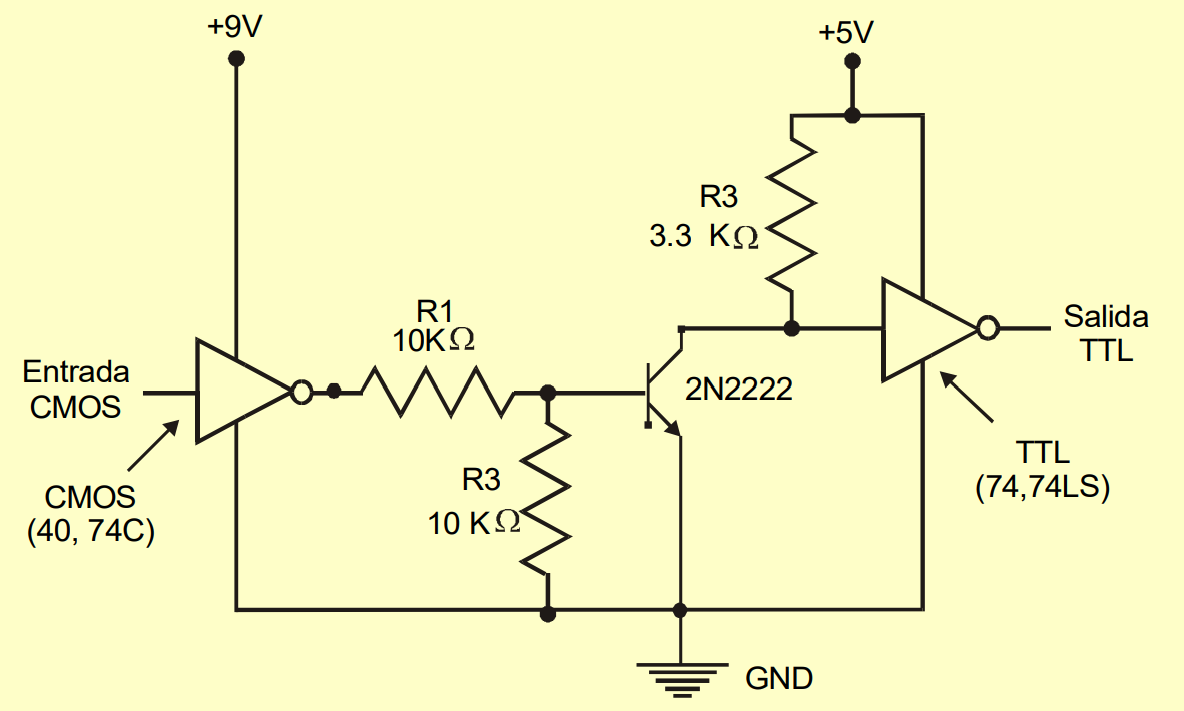
\includegraphics[scale = 0.2]{img/CMOSTTLTrans.png}
		\caption{Interfaz de CMOS a TTL con transistor \cite{Ladelex}}
		\label{fig:CMOSTTLTrans}
	\end{figure}
	
	\section{Sistema desarrollado}
	
	\subsection{Experimento 1}
	En este experimento es necesario modificar y dimensionar el circuito de la Figura \ref{fig:Circuito1}, además se deben dimensionar las resistencias que se muestran en dicho circuito, para esto se utilizará la Ecuación \ref{eqn:CRE1}:
	
	\begin{equation}
		V_{I} = \frac{R_{2}*V_{DD}}{R_{1} + R_{2}}, R_{1} = 1k\Omega
		\label{eqn:CRE1}
	\end{equation}
	
	\begin{figure}[htb]
		\centering
		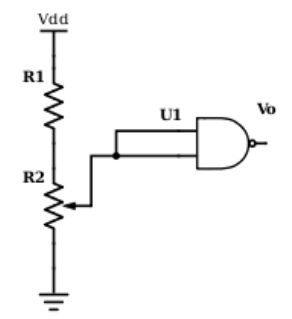
\includegraphics[scale = 0.3]{img/Circuito1.png}
		\caption{Circuito base para la medición del experimento 1}
		\label{fig:Circuito1}
	\end{figure}
	
	Utilizando la familia de tecnologías TTL, se tiene el circuito de la Figura \ref{fig:TTLC1}, la comparación entre sus valores teóricos y prácticos se encuentran en la Tabla \ref{tab:TvPTTL}.
	
	\begin{figure}[htb]
		\centering
		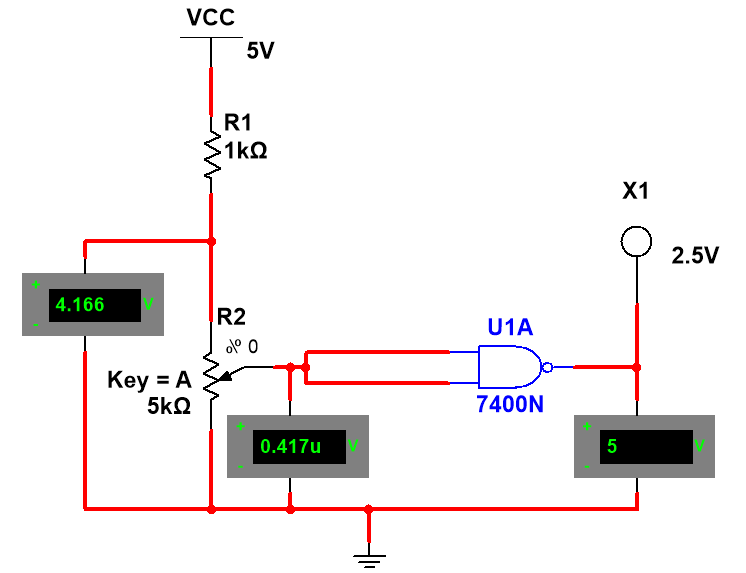
\includegraphics[scale = 0.4]{img/TTLC1.png}
		\caption{Circuito 1 adaptado TTL}
		\label{fig:TTLC1}
	\end{figure}
	
	\begin{table}[htb]
		\centering
		\begin{tabular}{lll}
			\hline
			NAND TTL  & Teórico (V) & Práctico (V)  \\
			\hline
			$V_{IH}$ & 5 - 2    & 4.999 - 2.549 \\
			$V_{IL}$ & 0.8 - 0  & 2.499 - 0.4 $\mu$ \\
			$V_{OH}$ & 5 - 3.4 & 5 \\
			$V_{OL}$ & 0.2 - 0  & 0 \\
		\end{tabular}
		\caption{Valores teóricos vs valores prácticos TTL}
		\label{tab:TvPTTL}
	\end{table}
	
	
	A su vez utilizando la familia de tecnologías CMOS, se tiene el circuito de la Figura \ref{fig:CMOSC1}, la comparación entre sus valores teóricos y prácticos se encuentran en la Tabla \ref{tab:TvPCMOS}.
	
	\begin{figure}[htb]
		\centering
		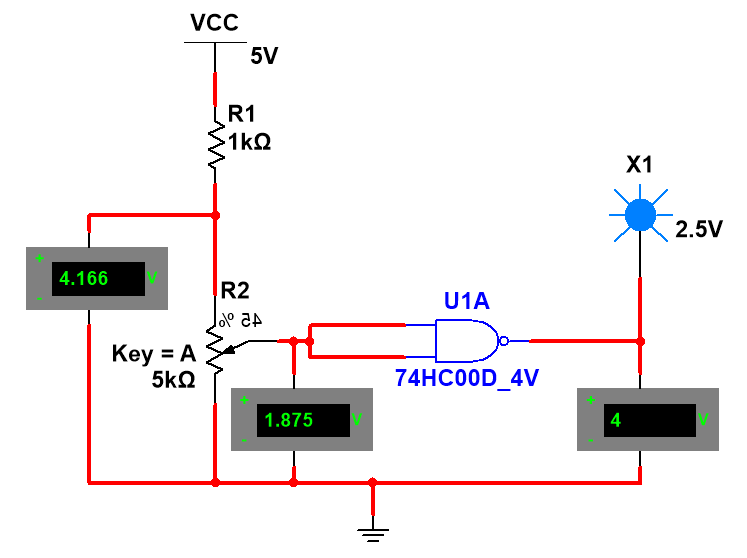
\includegraphics[scale = 0.4]{img/CMOSC1.png}
		\caption{Circuito 1 adaptado CMOS}
		\label{fig:CMOSC1}
	\end{figure}
	
	\begin{table}[htb]
		\centering
		\begin{tabular}{lll}
			\hline
			NAND TTL  & Teórico (V) & Práctico (V)  \\
			\hline
			$V_{IH}$ & 6 - 2    & 4.545 - 2.045 \\
			$V_{IL}$ & 2.1 - 0  & 2 - 0.455 $\mu$ \\
			$V_{OH}$ & 4 - 2.25 & 4 \\
			$V_{OL}$ & 0  & 0 \\
		\end{tabular}
		\caption{Valores teóricos vs valores prácticos CMOS}
		\label{tab:TvPCMOS}
	\end{table}
	
	\subsection{Experimento 2}
	
	Para este experimento se desea desarrollar la función que se muestra en la Ecuación \ref{eqn:FE2}, donde $\uparrow$ denota la operación NAND.
	
	\begin{equation}
		F = (A \uparrow B) \cdot C + (A \oplus C)
		\label{eqn:FE2}
	\end{equation}
	
	Por lo que el primer paso a realizar será obtener la tabla de verdad de la misma.
	
	\begin{table}[!htb]
		\centering
		\begin{tabular}{|c|c|c|c|c|c||c|}
			\hline
			A & B & C & $A \uparrow B$ & $(A \uparrow B) \cdot C$ & $A \oplus C$ & F \\
			\hline
			\hline
			0 & 0 & 0 & 1              & 0                        & 0            & 0 \\
			\hline
			0 & 0 & 1 & 1              & 1                        & 1            & 1 \\
			\hline
			0 & 1 & 0 & 1              & 0                        & 0            & 0 \\
			\hline
			0 & 1 & 1 & 1              & 1                        & 1            & 1 \\
			\hline
			1 & 0 & 0 & 1              & 0                        & 1            & 1 \\
			\hline
			1 & 0 & 1 & 1              & 1                        & 0            & 1 \\
			\hline
			1 & 1 & 0 & 0              & 0                        & 1            & 1 \\
			\hline
			1 & 1 & 1 & 0              & 0                        & 0            & 0 \\
			\hline
		\end{tabular}
		\caption{Tabla de verdad de la Ecuación \ref{eqn:FE2}}
		\label{tab:TVE2}
	\end{table}
	
	Explicación del diseño.
	
	\begin{figure}[!htb]
		\centering
		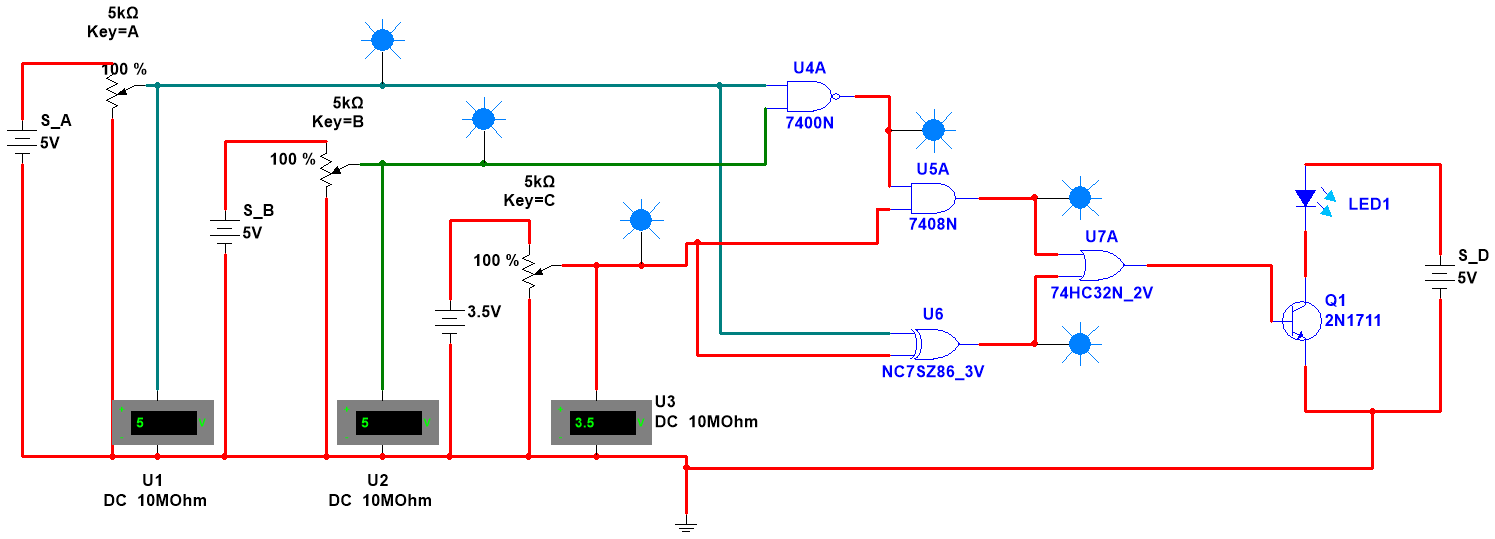
\includegraphics[scale = 0.215]{img/FuncionIterfaz.png}
		\caption{Circuito diseñado para desarrollar la Ecuación \ref{eqn:FE2}}
		\label{fig:CFI}
	\end{figure}
	
	\subsection{Experimento 3}
	
	Se desea diseñar un sumador completo de 2 bits a partir de un sumador completo de 1 bit sin el uso de la compuerta XOR, esta se puede desarrollar mediante el uso de compuertas más simples (NOT, OR, AND) como se observa en la Figura \ref{fig:XORSimple}. La tabla de verdad de un sumador completo de 1 bit se puede observar en la Tabla \ref{tab:TVSC1B} y su circuito se observa en la Figura \ref{fig:SC1B}.
	
	\begin{figure}[htb]
		\centering
		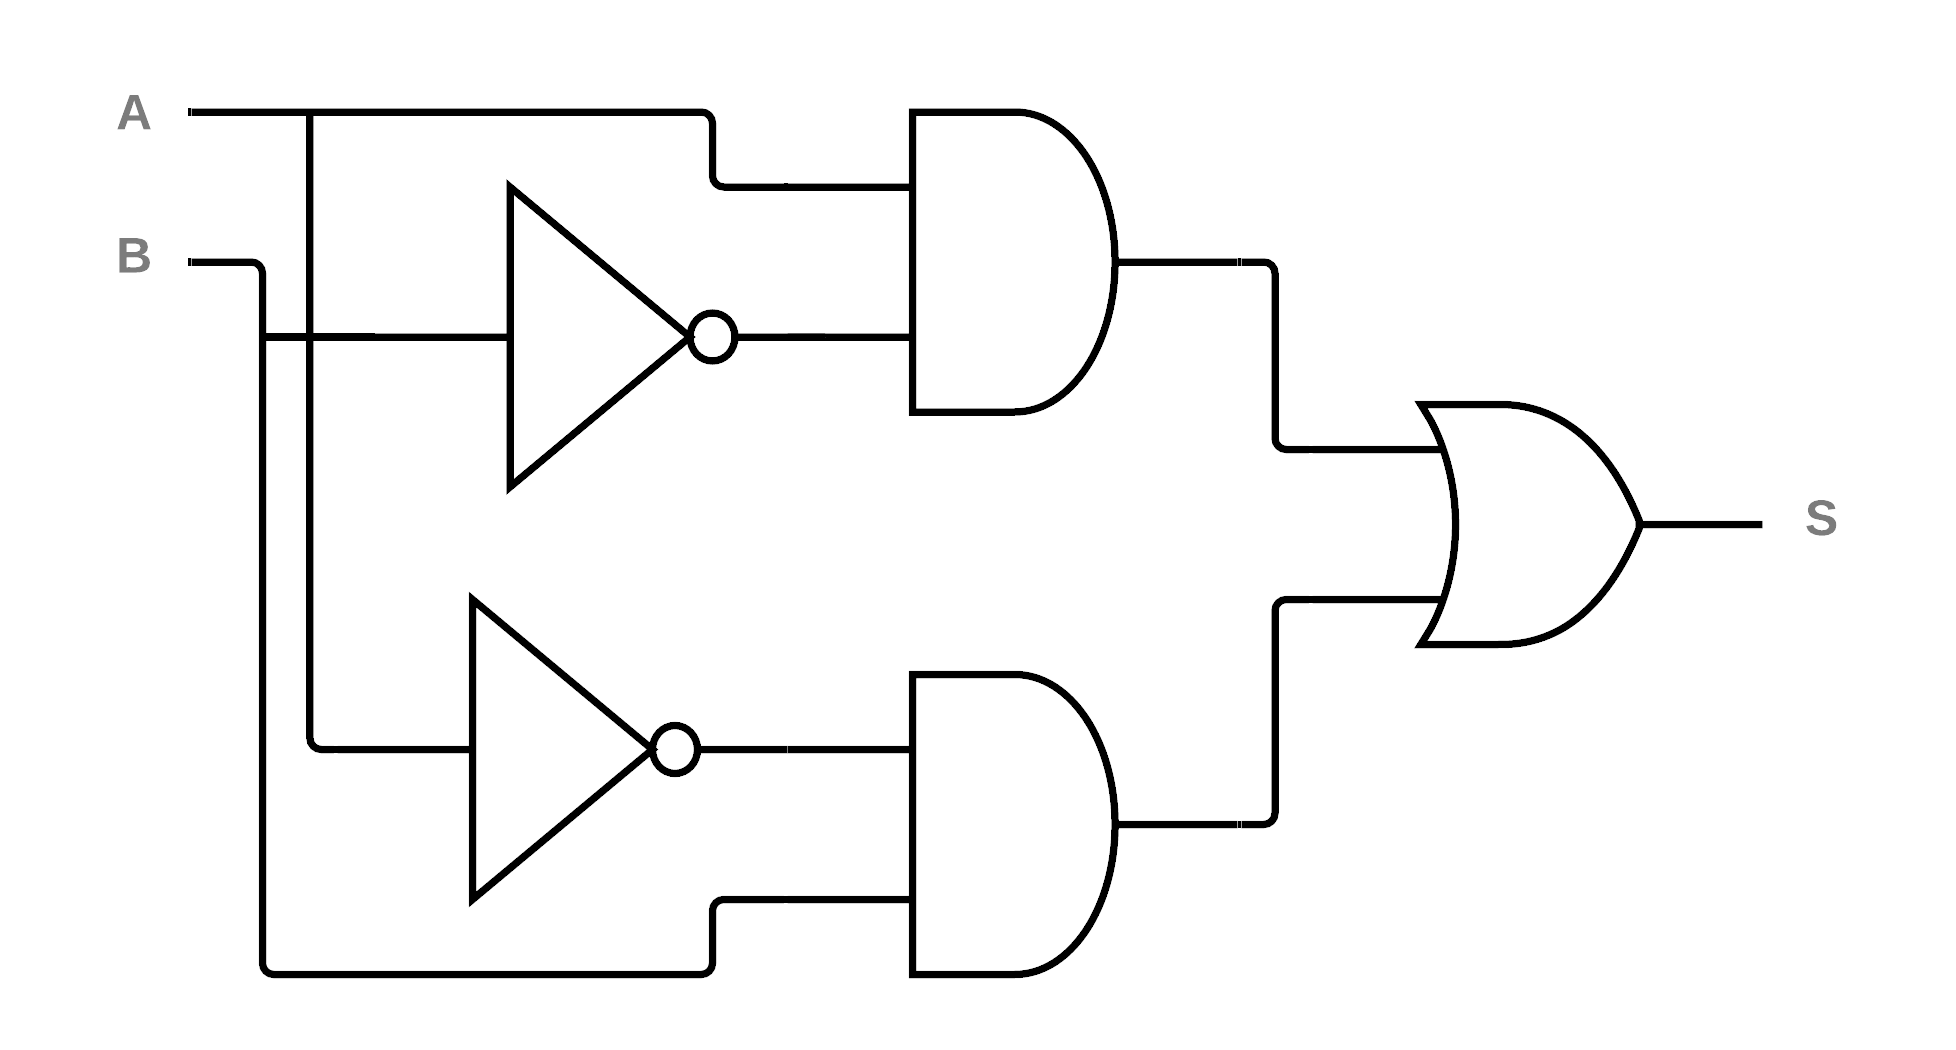
\includegraphics[scale = 0.1]{img/XORSimple.png}
		\caption{Compuerta XOR a partir de compuertas NOT, AND y OR.}
		\label{fig:XORSimple}
	\end{figure}
	
	\begin{table}[htb]
		\centering
		\scalebox{1.5}{
			\begin{tabular}{|c|c|c||c|c|}
				\hline
				A & B & $C_{in}$ & $C_{out}$ & S\\
				\hline
				\hline
				0 & 0 & 0 & 0 & 0 \\
				\hline
				0 & 0 & 1 & 0 & 1 \\
				\hline
				0 & 1 & 0 & 0 & 1 \\
				\hline
				0 & 1 & 1 & 1 & 0 \\
				\hline
				1 & 0 & 0 & 0 & 1 \\
				\hline
				1 & 0 & 1 & 1 & 0 \\
				\hline
				1 & 1 & 0 & 1 & 0 \\
				\hline
				1 & 1 & 1 & 1 & 1 \\
				\hline
		\end{tabular}}
		\caption{Tabla de verdad sumador completo de 1 bit}
		\label{tab:TVSC1B}
	\end{table}
	
	\begin{figure}[!htb]
		\centering
		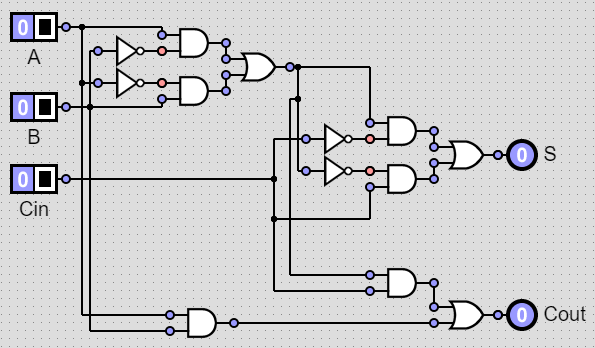
\includegraphics[scale = 0.5]{img/SC1B.png}
		\caption{Sumador completo de 1 bit con compuertas lógicas}
		\label{fig:SC1B}
	\end{figure}
	
	\begin{table}[!htb]
		\centering
		\scalebox{1.5}{
			\begin{tabular}{|c|c|c||c|c|c|}
				\hline
				A & B & $C_{in}$ & $C_{out}$ & Sd & Su\\
				\hline
				\hline
				0 & 0 & 0 & 0 & 0 & 0 \\
				\hline
				0 & 0 & 1 & 0 & 0 & 1 \\
				\hline
				0 & 1 & 0 & 0 & 1 & 1 \\
				\hline
				0 & 1 & 1 & 1 & 0 & 0 \\
				\hline
				1 & 0 & 0 & 0 & 1 & 1 \\
				\hline
				1 & 0 & 1 & 1 & 0 & 0 \\
				\hline
				1 & 1 & 0 & 1 & 1 & 0 \\
				\hline
				1 & 1 & 1 & 1 & 1 & 1 \\
				\hline
		\end{tabular}}
		\caption{Tabla de verdad sumador completo de 2 bits}
		\label{tab:TVSC2B}
	\end{table}
	
	\begin{figure}[!htb]
		\centering
		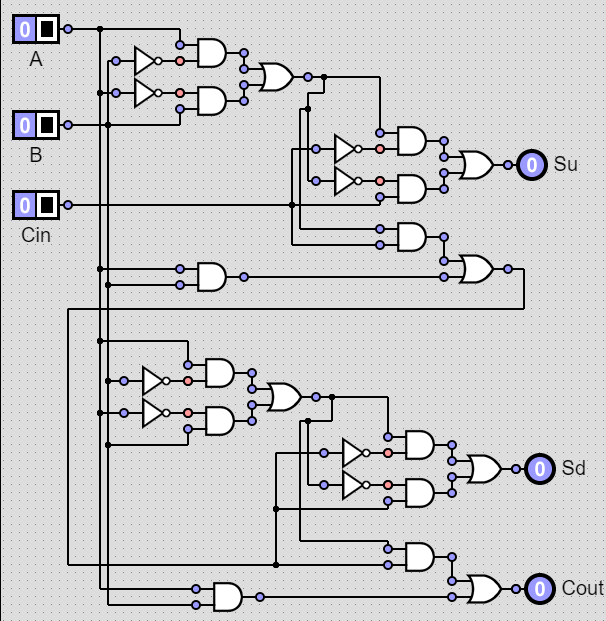
\includegraphics[scale = 0.5]{img/SC2B.png}
		\caption{Sumador completo de 2 bits con compuertas lógicas}
		\label{fig:SC2B}
	\end{figure}
	
	Además es necesario desarrollar el mismo a nivel de chip sin utilizar la compuerta XOR. Es por esto que el sistema que se desarrolló para el sumador de 1 bit se muestra en la Figura \ref{fig:Sumador1B}, este se compone de un de un bloque que se puede observar más detalladamente en la Figura \ref{fig:Sumador1BInside}, como se puede notar este se contiene a su vez de dos bloques $XOR$ donde cada uno está compuesto de compuertas lógicas básicas como AND, NOT y OR y se detallan en la Figura \ref{fig:XORInside}.
	
	\begin{figure}[!htb]
		\centering
		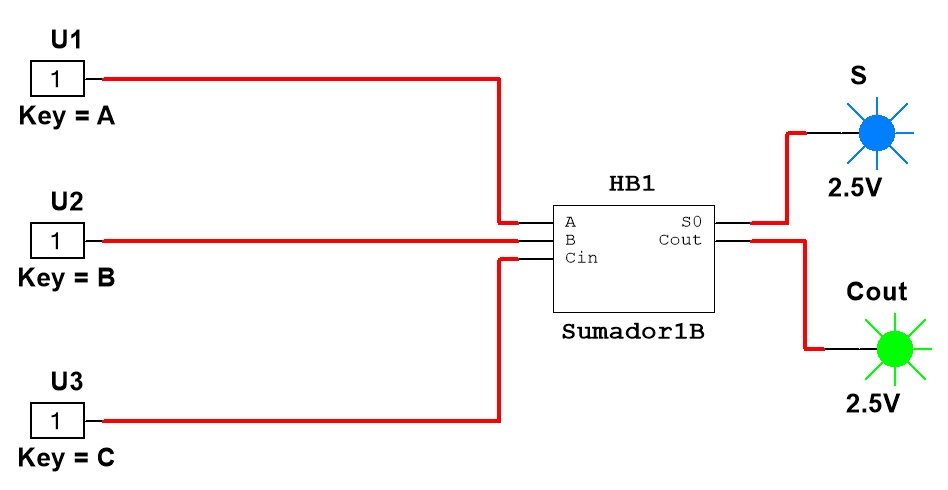
\includegraphics[scale = 0.35]{img/Sumador1B.png}
		\caption{Sumador de 1 bit}
		\label{fig:Sumador1B}
	\end{figure}
	
	\begin{figure}[!htb]
		\centering
		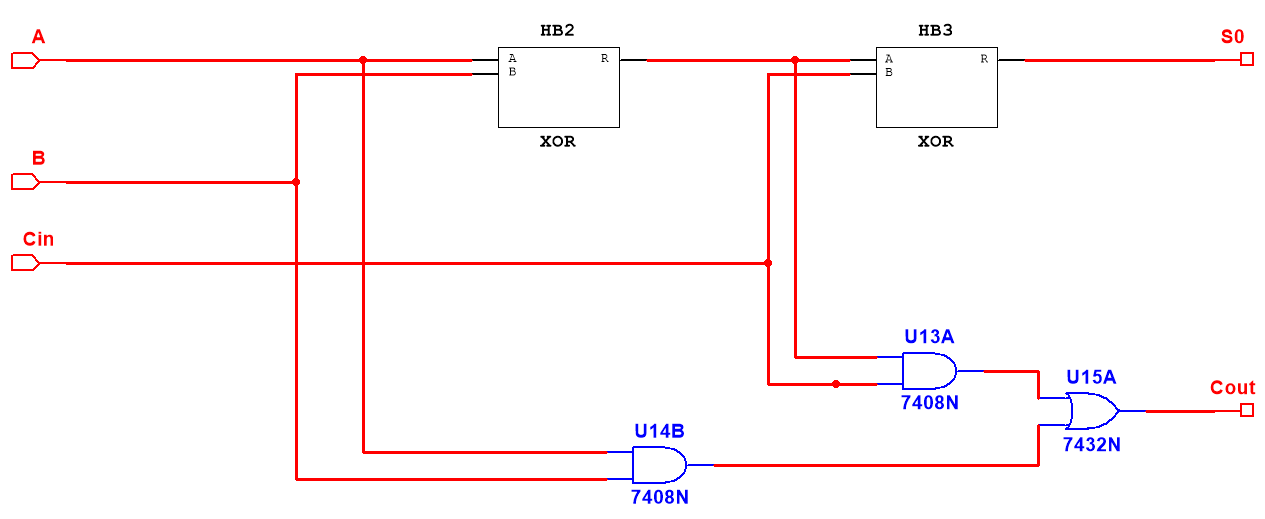
\includegraphics[scale = 0.26]{img/Sumador1BInside.png}
		\caption{Bloque del sumador de 1 bit}
		\label{fig:Sumador1BInside}
	\end{figure}
	
	\begin{figure}[!htb]
		\centering
		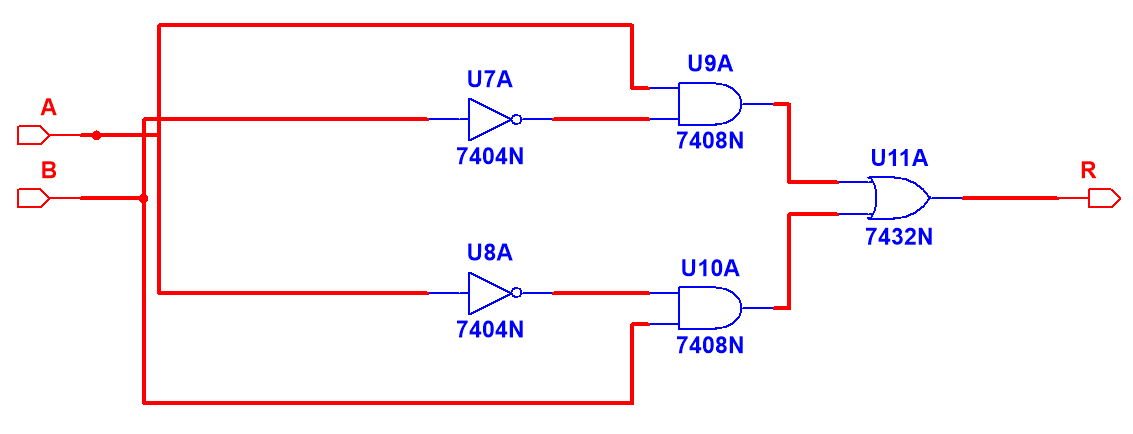
\includegraphics[scale = 0.28]{img/XORInside.png}
		\caption{Compuerta XOR desarrollada mediante chips de compuertas básicas}
		\label{fig:XORInside}
	\end{figure}
	
	Para el sumador de 2 bits se realizó un análisis similar, este se puede componer de dos sumadores de 1 bit cada uno, es por esto que como se observa en la Figura \ref{fig:Sumador2B} contiene dos bloques, la información detallada de estos se puede observar en las Figuras \ref{fig:Sumador1B}, \ref{fig:Sumador1BInside} y \ref{fig:XORInside}, ya que se aplicó un diseño modular para el sumador de 1 bit y estos se utilizaron para desarrollar en el sumador de 2 bits.
	
	\begin{figure}[!htb]
		\centering
		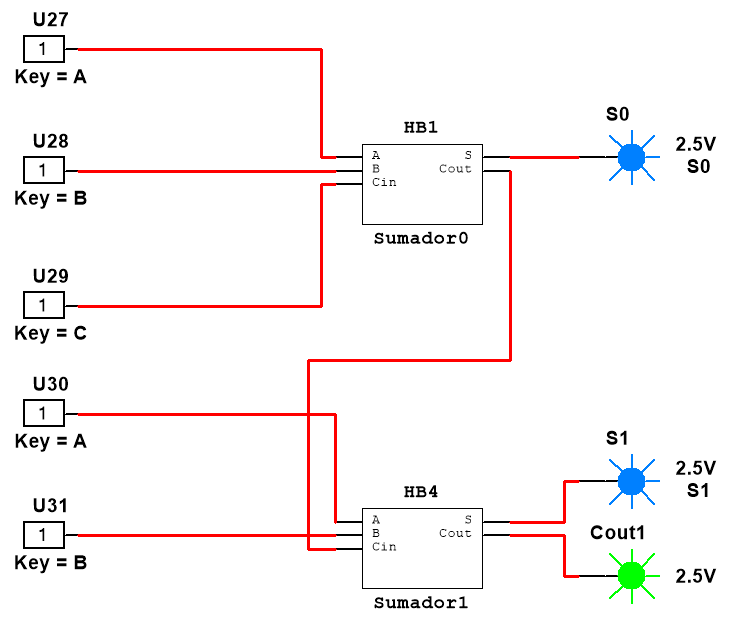
\includegraphics[scale = 0.4]{img/Sumador2B.png}
		\caption{Sumador de 2 bits}
		\label{fig:Sumador2B}
	\end{figure}
	
	\section{Análisis de resultados}
	\subsection{Experimento 1}
	En este caso como se puede apreciar en las Tablas \ref{tab:TvPTTL} y \ref{tab:TvPCMOS}, los valores teóricos y prácticos difieren mucho unos de los otros, se pueden asignar estas diferencias al uso de un simulador dado que este funciona con comportamientos ideales y/o limitados, con medidas muy distantes de la realidad. Uno de las observaciones mas importantes es que no se aprecia con claridad la región de la compuerta con comportamiento inestable, debido al cambio de funcionamiento de región de operación.
	
	\subsubsection{$V_{IH}$}
	En el caso de la tecnología TTL los valores teóricos están dentro del rango de 5V a 2V, pero en la práctica están en el rango de 4.99V a 2.549V. 
	\\
	Para el caso de la tecnología CMOS se muestra una diferencia mas significativa, dado que los valores en este estado son de 6V a 2V en cuanto a los valores teóricos, pero según las mediciones con el simulador estos valores son 4.545V a 2.045V, acá vemos una perdida de 1.5V aproximadamente hacia el límite superior. 
	
	\subsubsection{$V_{IL}$}
	En la compuerta TTL podemos apreciar quizás el caso mas marcado de todo el cuadro,  los valores prácticos de funcionamiento están en el rango de 0.8V a 0V, pero la práctica (simulación) nos indica que estos valores están en el rango de 2.499V a 0.4$\mu$V lo que supone una perdida en el funcionamiento real, dado que según la teoría, los valores dentro del rango de 2V a 0.8V deberían considerarse valores inciertos, pero como resultados de simulación nos indica que aun estos deben considerarse como estados de "operación" de la compuerta.
	\\
	En el caso de la CMOS el comportamiento se acerca un poco al ideal, dada la peculiaridad que la compuerta CMOS tiene "definida" el rango de cambio, podemos observar que la sección de incertidumbre es de apenas 0.1V.
	
	\subsubsection{$V_{OH}$}
	Para el caso de la familia TTL, al igual que el caso anterior se ve un desfase en los rangos teóricos y prácticos, pero con la diferencia que la salida nos muestra un resultado único, en este estado la salida en alto solo muestra 5V, siendo contrario a la teoría que nos da un rango de valores, que van desde los 5V a los 3.4V
	\\
	Lo mismo se puede apreciar en la familia CMOS que a pesar de la gran diferencia de valores que se presenta, de igual manera se tiene un unico valor de salida en la practica.
	
	\subsubsection{$V_{OL}$}
	Para la familia TTL el cambio no es relavante, de igual manera que para la familia CMOS
	
	
	Para ambos experimentos se utilizaron resistencias de 1K$\omega$ y un potenciómetro de 5k$\omega$, la primer resistencia se encuentra de manera experimental, dado que según los datos de las compuertas, la corriente de entrada es de 50 mA para ambos casos lo que nos deja una resistencia de 10$\omega$ sin embargo no muestra una caída de tensión significativa para los propósitos del experimento. Por lo cual se sustituye con la resistencia anteriormente mencionada
	
	\subsection{Experimento 2}
	Para este experimento se utilizan dos cosas fundamentales, primeramente se realiza la investigación de las compuertas de la serie 7xxx de la tecnología CMOS la cual nos permite una conexión directa con la familia TTL, gracias a sus pines compatibles con dicha familia. Luego, como podemos observar en la figura \ref{fig:CMOSTTL}, se nos permite conectar a ambas familias de forma directa, esto sumado a que los valores de tensión de la familia CMOS están dentro de los valores de la familia TTL, por lo que no se ve directamente afectada pro dicha conexión. Se hace la aclaración que se pudo escoger la conexion Pull-Up o Pull-Down para dicha interfaz, pero esto significa un gasto en componentes que no es deseado en los proyectos. 
	
	\subsection{Experimento 3}
	
	En el caso del experimento 3 se desarrolló para el caso del sumador de 1 bit dos versiones, el primero desde el una versión gráfica de compuertas lógicas como el que se observa en la Figura \ref{fig:SC1B} además de una versión a nivel de chip como el de la Figura \ref{fig:Sumador1B}. A nivel de compuertas gráficas mediante el simulador en línea se obtuvo la tabla de verdad que se observa en la Figura \ref{fig:TSC1B}, al comparar esta tabla de valores simulados con la Tabla \ref{tab:TVSC1B} que presenta los resultados teóricos podemos observar que sus resultados son los mismos, por lo que se demuestra que esta simulación presenta un correcto funcionamiento.
	
	Además al realizar las pruebas en la versión simulada mediante chips también se llegó a los mismos resultados al ingresar cada entrada una a una, lo cual nos indica que también funciona correctamente.
	
	\begin{figure}[htb]
		\centering
		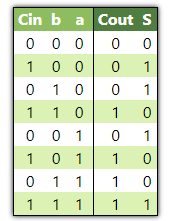
\includegraphics[scale = 0.7]{img/TSC1B.png}
		\caption{Resultado simulador en línea sumador completo de 1 bit}
		\label{fig:TSC1B}
	\end{figure}
	
	Por otro lado para el caso del sumador de 2 bis también se desarrollaron dos versiones, el primero desde el una versión gráfica de compuertas lógicas como el que se encuentra en la Figura \ref{fig:SC2B} además de una versión a nivel de chip como el de la Figura \ref{fig:Sumador2B}. A nivel de compuertas gráficas mediante el simulador en línea se obtuvo la tabla de verdad que de la Figura \ref{fig:TSC2B}, al comparar esta tabla de valores simulados con la Tabla \ref{tab:TVSC2B} que presenta los resultados teóricos podemos observar que sus resultados son los mismos, por lo que se demuestra que esta simulación presenta un correcto funcionamiento.
	
	Además al realizar las pruebas en la versión simulada mediante chips también se llegó a los mismos resultados al ingresar cada entrada una a una, lo cual nos confirma el correcto funcionamiento de esta.
	
	\begin{figure}[htb]
		\centering
		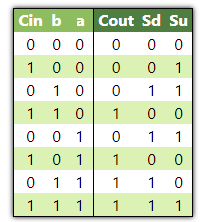
\includegraphics[scale = 0.7]{img/TSC2B.png}
		\caption{Resultado simulador en línea sumador completo de 2 bits}
		\label{fig:TSC2B}
	\end{figure}
	
	Cabe destacar que en las Figuras \ref{fig:TSC1B} y \ref{fig:TSC2B} en las entradas el LSB (Least Significant Bit) es el que se encuentra en la primer columna y el MSB (Most-significant bit) en la tercera.
	
	\section{Conclusiones}
	
	En el pasado realizar la conexión entre dos familias distintas como lo son las tecnologías TTL y CMOS requería de utilizar distintas interfaces como las de las Figuras \ref{fig:TTLCMOSRes}, \ref{fig:TTLCMO74HC}, \ref{fig:TTLCMOSColAb}, \ref{fig:TTLCMOSTrans}, \ref{fig:CMOSTTL}, \ref{fig:CMOSTTLRes}, \ref{fig:CMOSTTLBuff}, \ref{fig:CMOSTTL40} y \ref{fig:CMOSTTLTrans}, pero con el desarrollo de la tecnología HC (High speed CMOS), que es un caso especial de la tecnología CMOS no es necesario realizar una interfaz entre estos, ya que la serie HC tiene niveles lógicos compatibles con la tecnología TTL \cite{Unicrom}.
	
	Las compuertas lógicas son fundamentales para realizar distintos circuitos en electrónica y se pudo comprobar mediante la realización de sumadores de 1 bit, 2 bits y funciones más complejas como \ref{eqn:FE2}. Demostrando que es escalable ya que el sumador de 2 bits se realizó mediante el diseño modular utilizando el sumador de 1 bit, y este a su vez podría escalarse para implementar un sumador de 4 o n bits.
	
	El uso de herramientas de simulación supone en muchas ocasiones estar anuentes a comportamientos ideales, o fallas en la programación que puede afectar el funcionamiento de nuestro modelo, en este caso la región de incertidumbre de las compuertas no pudo ser medida dado el comportamiento ideal del simulador, el cambio de estado no se da de manera escalonada, sino de manera continua ascendente o descendente según sea el caso. Por ello se debe tener en cuenta que las simulaciones son un paso mas del método de diseño modular, y no debería ser la ultima opción antes de sacar un dispositivo a producción, las simulaciones nos guían a través del problema para encontrar la solución, pero no son la respuesta definitiva, sin duda alguna debemos prepararnos para hacer prototipos y verificar el funcionamiento del modelo de forma física. 
	
	\section{Bibliografía}
	
	\begin{thebibliography}{1}
		
		\bibitem{74HC00D} “74HC00D pdf, 74HC00D description, 74HC00D datasheets, 74HC00D view ::: ALLDATASHEET :::”, Pdf1.alldatasheet.com, 2021. [En línea]. Disponible: \url{https://pdf1.alldatasheet.com/datasheet-pdf/view/344388/NXP/74HC00D.html}. [Accesado: 23- Feb- 2021].
		
		\bibitem{74HC32N} “74HC32N pdf, 74HC32N description, 74HC32N datasheets, 74HC32N view ::: ALLDATASHEET :::”, Pdf1.alldatasheet.com, 2021. [En línea]. Disponible: \url{https://pdf1.alldatasheet.com/datasheet-pdf/view/536726/PHILIPS/74HC32N.html}. [Accesado: 23- Feb- 2021].
		
		\bibitem{SDLS025D} Ti.com, 2021. [En línea]. Disponible: \url{https://www.ti.com/lit/ds/sdls025d/sdls025d.pdf}. [Accesado: 23- Feb- 2021].
		
		\bibitem{NC7SZ86} Onsemi.com, 2021. [En línea]. Disponible: \url{https://www.onsemi.com/pub/Collateral/NC7SZ86-D.PDF}. [Accesado: 23- Feb- 2021].
		
		\bibitem{Intel} “fan-in and fan-out”, Intel.com, 2021. [En línea]. Disponible: \url{https://www.intel.com/content/www/us/en/programmable/quartushelp/13.0/mergedProjects/reference/glossary/def_fan.htm}. [Accesado: 23- Feb- 2021].
		
		\bibitem{NI} “Interfacing TTL and CMOS Circuits - National Instruments”, Knowledge.ni.com, 2021. [En línea. Disponible: \url{https://knowledge.ni.com/KnowledgeArticleDetails?id=kA03q000000YHhjCAG&l=en-US}. [Accesado: 18- Feb- 2021].
		
		\bibitem{Ladelex} J. Jiménez, “Interfases entre TTL y CMOS”, Ladelec.com, 2021. [En línea]. Disponible: \url{http://www.ladelec.com/teoria/electronica-digital/369-interfases-entre-ttl-y-cmos}. [Accesado: 22- Feb- 2021].
		
		\bibitem{LOGICBUS} “Las Compuertas Lógicas y sus Operaciones Lógicas (AND, OR, NOT, NAND, NOR, XOR, XNOR)”, Logicbus.com.mx, 2021. [En línea]. Disponible: \url{https://www.logicbus.com.mx/compuertas-logicas.php}. [Accesado: 18- Feb- 2021].
		
		\bibitem{Unicrom} “Niveles lógicos (alto, bajo, 0, 1, Low, High) - Electrónica Unicrom”, Electrónica Unicrom, 2021. [En línea]. Disponible: \url{https://unicrom.com/niveles-logicos-alto-bajo-0-1-low-high/}. [Accesado: 18- Feb- 2021].
		
		\bibitem{SN7408N} “SN7408N pdf, SN7408N Descripcion, SN7408N datasheets, SN7408N Vista ::: ALLDATASHEET :::”, Pdf1.alldatasheet.es, 2021. [En línea]. Disponible: \url{https://pdf1.alldatasheet.es/datasheet-pdf/view/177352/TI/SN7408N.html}. [Accesado: 23- Feb- 2021].
		
		\bibitem{UnicromS} “Sumador binario completo de 1 bit - Electrónica Unicrom”, Electrónica Unicrom, 2021. [En línea]. Disponible: \url{https://unicrom.com/sumador-binario-completo-de-1-bit}. [Accesado: 22- Feb- 2021].
		
	\end{thebibliography}
	
\end{document}